\documentclass[../main/main.tex]{subfiles}

\raggedbottom

\makeatletter
\renewcommand{\@chapapp}{\'Electrocin\'etique -- chapitre}
\makeatother

\toggletrue{student}

\begin{document}
\setcounter{chapter}{4}

\chapter{Circuits \'electriques en r\'egime sinuso\"idal forc\'e}

Jusque-là en électrocinétique, nous avons étudié la réponse d'un circuit
(c'est-à-dire la tension de sortie) de systèmes linéaires soumis à une
modification rapide de l'entrée (régime libre et échelon montant) d'une valeur
constante à une autre. Nous avons alors observé la présence d'un régime
\textbf{transitoire} suivi d'un régime \textbf{permanent \underline{constant}}.
Dans ce chapitre, nous allons voir la réponse d'un circuit à une entrée
\textbf{sinusoïdale}, qui donnera lieu à un régime transitoire suivi d'un régime
\textbf{permanent \underline{sinusoïdal}}. D'une manière générale, on se
concentre sur la réponse du système une fois le régime permanent établi. On
définit donc

\begin{defi}[label=def:rsf]{Régime sinusoïdal forcé}
    On appelle \textbf{régime sinusoïdal forcé} le régime permanent d'un circuit
    électrique soumis à une entrée sinusoïdale. Dans tout le chapitre, on
    supposera donc que l'entrée est allumées depuis une durée suffisamment
    longue pour considérer que le régime transitoire est terminé.
\end{defi}

\section{Circuit RC série en RSF}
\subsection{Présentation}
Soit le circuit RC série, avec $e(t) = E_0\cos(\wt)$.
\begin{center}
    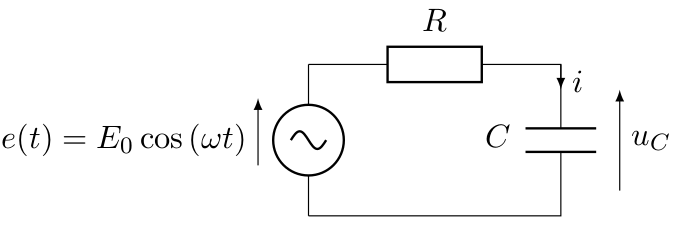
\includegraphics[width=.5\linewidth]{rc_rsf}
\end{center}
On en a maintenant l'habitude, on va appliquer la loi des mailles sur le circuit
et utiliser les relations courant-tension en fonction des bonnes conventions~:
\begin{gather*}
    u_C + u_R = e(t)
    \Leftrightarrow
    u_C + Ri = e(t)
    \Leftrightarrow
    u_C + RC \dv{u_C}{t} = e(t)\\
    \Leftrightarrow
    \boxed{ \dv{u_C}{t} + \frac{1}{\tau}u_C = \frac{1}{\tau}E_0\cos(\wt)}
\end{gather*}
avec $\tau = RC$ la constante de temps.

Résoudre cette équation différentielle demande comme précédemment de trouver la
solution homogène et la solution particulière. La solution homogène est la
solution de
\begin{gather*}
    \dv{u_C}{t} + \frac{1}{\tau}u_C = 0
\end{gather*}
c'est-à-dire
\begin{gather*}
    u_{C,h}(t) = K\exp \left( - \frac{t}{\tau} \right)
\end{gather*}
Pour la solution particulière, \textbf{on admet} qu'elle est de la forme
\begin{gather*}
    u_{C,p}(t) = U\cos(\wt + \f)
\end{gather*}
ce qui donne une solution générale
\[\boxed{u_C(t) = K\exp \left( - \frac{t}{\tau} \right) + U\cos(\wt + \f)}\]

\begin{ror}[label=ror:CIounon, hand]{Attention}
    $K$ dépend des conditions initiales, mais\smallbreak
    \centering\large $U$ et $\f$ dépendent du circuit (ici, $R$, $C$, $\w$ et $E_0$).
\end{ror}

\subsection{Réponse d'un système en RSF}
En supposant le régime permanent établi (définition du RSF), on a donc~:
\begin{prop}[label=prop:sortiersf, heart]{forme de la réponse d'un système en RSF}
    Pour un signal d'entrée
    \[e(t) = E_0 \cos(\wt)
    \quad(\text{ou}\quad
    \eta(t) = \eta_0\cos(\wt))\]
    les différentes tensions et intensités dans le circuit oscilleront \textbf{à
    la même pulsation $\w$}, et seront de la forme
    \[u(t) = U\cos(\wt+\f_u)
    \qet
    i(t) = I\cos(\wt+\f_i)\]
    où $U$ et $\f_{u,i}$ sont deux constantes dépendant du système et de l'excitation
    $\w$.
\end{prop}
\begin{rror}{\includehand{-90}{.8cm}}
    L'objectif de ce chapitre est de donc de savoir déterminer $U$ et $\f$.
\end{rror}
\vspace{-30pt}
\subsection{Passage en complexes}
Une méthode de résolution est d'introduire la formule $U\cos(\wt+\f)$ dans
l'équation différentielle et de rechercher $U$ et $\f$. Si c'est possible, c'est
très calculatoire (cf.\ cours de maths). L'utilisation des nombres complexes
permet de réduire drastiquement cette difficulté. \bigbreak

\begin{rdemo}{Méthode}
    Pour cela, on remplace $u(t)$ et $e(t)$ par leur forme complexe~:

    \begin{gather*}
        \ul{u_C} = \ul{U}\exr^{\jj\wt}
        \qavec
        \ul{U} = U\exr^{\jj\f}
        \qet
        \ul{e} = E_0\exr^{\jj\wt}
    \end{gather*}

    Pour revenir aux valeurs réelles après calcul, on prendra donc
    \begin{gather*}
        U_C = \left| \ul{U_C} \right|
        \qet
        \f = \arg(\ul{U_C})
    \end{gather*}
\end{rdemo}

\begin{rexem}{Application}
    À partir de l'équation différentielle, on remplace les valeurs réelles par les
    valeurs complexes, en se rappelant que dériver en complexes revient à multiplier
    par $\jj\w$~:
    \begin{align*}
        \tau\dot{\ul{u_C}} + \ul{u_C} &= \ul{e}\\
        \Leftrightarrow
        RC\jj\w\ul{U}\cancel{\exr^{\jj\wt}} + \ul{u_C} &=
        E_0\cancel{\exr^{\jj\wt}}\\
        \Leftrightarrow
        \ul{U_C} \left( RC\jj\w + 1 \right) &= E_0\\
        \Leftrightarrow
        \Aboxed{
        \ul{U_C} &= \frac{E_0}{1 + \jj RC\w}}
    \end{align*}
\end{rexem}
    Il ne reste plus qu'à prendre le module de $\ul{U_C}$ pour avoir l'amplitude
    réelle, et l'argument de $\ul{U_C}$ pour avoir la phase à l'origine des
    temps.
\begin{rrapp}{Rappel}
    Pour cela, on rappelle que pour $\ul{z} \in \Cb$ tel que $\ul{z} = x + \jj
    y$, on a
    \[ \left| \ul{z} \right| = \sqrt{x^2 + y^2}\]
    Notamment, le module d'un nombre réel pur est égal à sa valeur absolue,
    et celui d'un nombre complexe pur à la valeur absolue de sa partie
    imaginaire. \bigbreak
    De plus, \textbf{le module d'un rapport est égal au rapport des modules}~:
    $\forall (\ul{z_1}, \ul{z_2}) \in \Cb^2$,
    \[ \left| \frac{\ul{z_1}}{\ul{z_2}} \right| =
    \frac{|\ul{z_1}|}{|\ul{z_2}|}\]
    \vspace*{-30pt}
\end{rrapp}
\begin{rexem}{Application}
    Ainsi,
    \begin{gather*}
        U_C
            = \left| \ul{U_C} \right|
            = \left| \frac{E_0}{1 + \jj RC\w} \right|
            = \frac{|E_0|}{|1 + \jj RC\w|}\\
    \end{gather*}
    \vspace*{-70pt}
\end{rexem}
\begin{rprop}{Résultat}
    \begin{gather*}
        \Leftrightarrow
        \boxed{
        U_C = \frac{E_0}{\sqrt{1+(RC\w)^2}}}
    \end{gather*}
\end{rprop}

On fait de même pour la phase, avec pour rappel~:
\begin{rrapp}{Rappel}
    Pour $\ul{z} \in \Cb$,
    \[\tan(\arg(\ul{z})) = \frac{\Im(\ul{z})}{\Re(\ul{z})}
    \qquad
    \cos(\arg(\ul{z})) = \frac{\Re(\ul{z})}{|\ul{z}|}
    \qquad
    \sin(\arg(\ul{z})) = \frac{\Im(\ul{z})}{|\ul{z}|}\]
    On aura notamment que l'argument d'un nombre réel positif est donc 0. On
    rappelle également que $\tan(-x) = -\tan(x)$. \bigbreak
    Mais encore, 
    \textbf{l'argument d'un rapport est égal à la différence des arguments}~:
    $\forall (\ul{z_1}, \ul{z_2}) \in \Cb^2$,
    \[ \arg\left( \frac{\ul{z_1}}{\ul{z_2}} \right) =
    \arg(\ul{z_1}) - \arg(\ul{z_2})\]
    \vspace*{-30pt}
\end{rrapp}
\begin{rexem}{Application}
    Ainsi,
    \begin{gather*}
        \f
            = \arg \left( \frac{E_0}{1+\jj RC\w} \right)
            = \underbrace{\arg(E_0)}_{=0} - \arg (1+\jj RC\w)
    \end{gather*}
    D'une manière générale, on utilisera l'expression de la tangente d'un
    argument \textbf{avant} de voir si on peut prendre l'arctangente de la
    tangente. 
    \begin{gather*}
        \tan(\f)
            = - \tan(\arg(1+\jj RC\w))
            = - \frac{RC\w}{1}
    \end{gather*}
\end{rexem}
\begin{rror}{Attention}
    Ça peut être une réponse acceptable dans certaines conditions, mais bien souvent
    on souhaite exprimer la phase directement. Dans ce cas, il faut faire attention
    au fait que
    \[\arctan(\tan(\theta)) = \theta \Leftrightarrow \theta \in \left] -
    \frac{\pi}{2}\,; \frac{\pi}{2} \right[\]
    Une manière de s'assurer de l'appartenance de $\theta$ à cet intervalle, il
    suffit de regarder le cosinus de
    $\theta$~: s'il est positif, alors on a en effet $\theta \in \left] -
    \frac{\pi}{2}\,; \frac{\pi}{2} \right[$. Ici,

    \begin{gather*}
        \cos(\arg(\f))
            = \frac{\Re(\arg(\f))}{|\ul{z}|}
            = \frac{1}{\sqrt{1 + (RC\w)^2}} > 0
    \end{gather*}
    donc on peut bien dire que $\arctan\tan(\f) = \f$.
\end{rror}
On remarquera que dès que la partie réelle d'un argument est positif, alors on
peut sans problème prendre l'arctangente de la tangente de l'argument.

\begin{rprop}{Résultat}
    Ainsi, on a finalement
    \[\boxed{\f = -\arctan(RC\w)}\]
    et la solution particulière est
    \begin{gather*}
        \boxed{u_C (t) = U_C\cos(\wt + \f)}\\
        \text{avec}\\
        \boxed{U_C = \frac{E_0}{\sqrt{1+(RC\w)^2}}}
        \qet
        \boxed{\f = -\arctan(RC\w)}
    \end{gather*}
\end{rprop}

\begin{NCrapp}[]{Remarque~: dépendance en $\w$}
    Comme on l'a vu, le signal de sortie sera à la même pulsation que le signal
    d'entrée, mais par cet exemple du circuit RC on note que la phase et
    l'amplitude \textbf{dépendent de la pulsation}.
\end{NCrapp}

\begin{instruc}[trans]{Transition}
    À partir de cet exemple, est-ce qu'on peut étendre l'utilisation des
    complexes pour le RSF aux lois de bases de l'électrocinétique~?
\end{instruc}

\section{Circuits électriques en RSF}
Comme au début de l'année, nous nous plaçons toujours dans l'Approximation des
Régimes Quasi-Stationnaires (ARQS), c'est-à-dire que pour un circuit de taille
$L$ alimenté par une source sinusoïdale de fréquence $f$, on doit avoir
\[\boxed{Lf \ll c}\]
avec $c$ la célérité de la lumière/des ondes électromagnétiques.

\subsection{Lois de l'électrocinétique}
\subsubsection{Loi des nœuds en RSF}
\begin{wrapfigure}[4]{R}{.5\linewidth}
    \vspace*{-40pt}
    \centering
    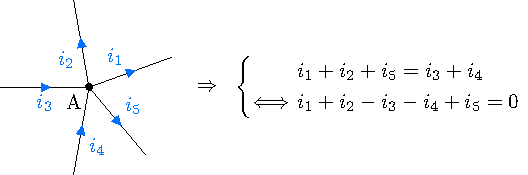
\includegraphics[width=\linewidth]{ldn}
\end{wrapfigure}
Soit un nœud où se rejoignent 5 branches. Dans l'ARQS, nous avions
la relation ci-contre. En RSF, les intensités sont sinusoïdales \textbf{et
de même pulsation} $\w$~: on aurait donc
\[
    i_1(t) = I_1\cos(\wt+\f_1)
    \qet
    i_2(t) = I_2\cos(\wt+\f_2)
    \qet
    …
\]

\begin{rprop}{Propriété}
    Ainsi, en passant en complexes, on aura
    \begin{gather*}
        \ul{i_1} + \ul{i_2} + \ul{i_5} = \ul{i_3} + \ul{i_4}
        \Leftrightarrow
        \boxed{\ul{I_1} + \ul{I_2} + \ul{I_5} = \ul{I_3} + \ul{I_4}}\\
        \text{avec}\quad
        \ul{i_k} = I_k\exr^{\jj\f_k}\exr^{\jj\wt}
        \qet
        \ul{I_k} = I_k\exr^{\jj\f_k}
    \end{gather*}
    \begin{center}
        \textbf{On a donc bien la même relation avec les grandeurs complexes et
        leurs amplitudes complexes}.
    \end{center}
\end{rprop}

\subsubsection{Loi des mailles}
\begin{wrapfigure}[4]{R}{.5\linewidth}
    \vspace*{-30pt}
    \centering
    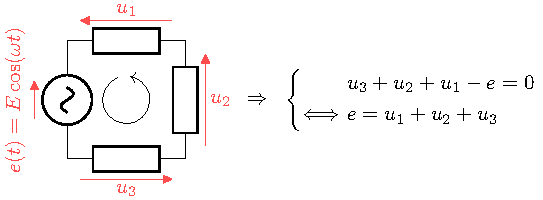
\includegraphics[width=\linewidth]{ldm_rsf}
\end{wrapfigure}
Soit une maille avec des dipôles quelconques, alimentée par une tension
sinusoïdale $e(t) = E\cos(\wt)$. Dans l'ARQS, nous avions la relation ci-contre.
En RSF, les tensions sont sinusoïdales \textbf{et de même pulsation} $\w$~: on
aurait donc
\[
    u_1(t) = U_1\cos(\wt+\f_1)
    \qet
    u_2(t) = U_2\cos(\wt+\f_2)
    \qet
    …
\]

\begin{rprop}{Propriété}
    Ainsi, en passant en complexes, on aura
    \begin{gather*}
        \ul{e} = \ul{u_1} + \ul{u_2} + \ul{u_3}
        \Leftrightarrow
        \boxed{\ul{E} = \ul{U_1} + \ul{U_2} + \ul{U_3}}\\
        \text{avec}\quad
        \ul{u_k} = U_k\exr^{\jj\f_k}\exr^{\jj\wt}
        \qet
        \ul{U_k} = U_k\exr^{\jj\f_k}
    \end{gather*}
    \begin{center}
        \textbf{On a donc bien la même relation avec les grandeurs complexes et
        leurs amplitudes complexes}.
    \end{center}
\end{rprop}

\subsection{Impédance et admittance complexes d'un dipôle passif}
\subsubsection{Définition}
En complexes, pour chaque dipôle on aura
\begin{align*}
    u(t) = U\cos(\wt+\f_u)
    &\qet
    i(t) = I\cos(\wt+\f_i)\\
    \Longrightarrow
    \ul{u}(t) = U\exr^{\jj(\wt+\f_u)} = U\exr^{\jj\f_u}\exr^{\jj\wt} =
    \ul{U}\exr^{\jj\wt}
    &\qet
    \ul{i}(t) = I\exr^{\jj(\wt+\f_i)} = I\exr^{\jj\f_i}\exr^{\jj\wt} =
    \ul{I}\exr^{\jj\wt}
\end{align*}
Ainsi, on peut aisément exprimer une relation courant-tension pour un dipôle
complexe, sous la forme classique $U = RI$ mais en complexes~: en effet, on peut
tout à fait calculer $\frac{\ul{u}}{\ul{i}}$ pour avoir une proportionnalité
entre les deux~: on appelle cette constante l'\textbf{impédance}, notée
$\ul{Z}$, et on a donc la \textbf{loi d'Ohm complexe}~:

\begin{rdefi}{Définition}
    \begin{minipage}{0.50\linewidth}
        \begin{gather*}
            \textbf{Loi d'Ohm complexe}\\
            \ul{u}(t) = \ul{Z}\ul{i}(t)
            \Leftrightarrow
            \boxed{\ul{U} = \ul{Z}\times\ul{I}}\\
            \Rightarrow
            \ul{Z}\quad\text{homogène à une résistance}
        \end{gather*}
    \end{minipage}
    \begin{minipage}{0.50\linewidth}
        \begin{center}
            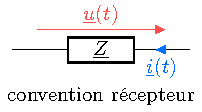
\includegraphics[width=.5\linewidth]{zdef}
        \end{center}
    \end{minipage}
\end{rdefi}

En tant que complexe, on peut prendre son module est son argument~:
\begin{itemize}
    \item Son module $Z = \left| \ul{Z} \right|$ est égal au rapport de
        l'amplitude de $u$ sur celle de $i$~:
        \[\boxed{ \left| \ul{Z} \right|
                = \frac{|\ul{u}|}{|\ul{i}|}
            = \frac{U}{I}
            }
        \]
    \item Son argument $\arg(\ul{Z})$ est égal à la différence de phase entre
        $\ul{u}$ et $\ul{i}$ (aussi appelée \textbf{déphasage}, voir Section
        ultérieure)~:
        \[\boxed{\arg(\ul{Z})
                = \arg \left( \frac{\ul{u}}{\ul{i}} \right)
            = \f_u - \f_i}
        \]
\end{itemize}

\begin{rdefi}{Définition}
    Assez naturellement, comme on avait la conductance égale à l'inverse d'une
    résistance, on peut définir l'inverse d'une impédance~: c'est
    l'\textbf{admittance complexe} $\ul{Y}$~:
    \[\boxed{\ul{Y}
        = \frac{1}{\ul{Z}} \Rightarrow \ul{I}
    = \ul{Y}\times\ul{U}}\]
\end{rdefi}

\vspace{-25pt}
\subsubsection{Impédances de bases}

Pour trouver les impédances des dipôles de base, on utilise leurs relations
courant-tension qu'on convertit en complexes, \textbf{en se souvenant de dériver
en complexes équivaut à multiplier par $\jj\w$}.

\begin{NCdefi}[width=\linewidth, tabularx={Y|Y|Y}, heart]
    {Définition~: impédances des dipôles de base}
    \textbf{Résistance} &
    \textbf{Inductance} &
    \textbf{Capacité}
    \\\hline
    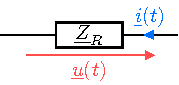
\includegraphics[width=\linewidth]{zr} &
    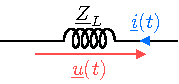
\includegraphics[width=\linewidth]{zl} &
    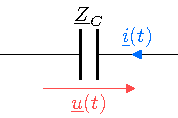
\includegraphics[width=\linewidth]{zc}
    \\\hline
    $\begin{aligned}
        u(t)             & = Ri(t)\\
        \Leftrightarrow
        \ul{u}(t)        & = R\ul{i}(t)\\
        \Leftrightarrow
        \Aboxed{\ul{Z}_R & = R}
    \end{aligned}$
                                           &
    $\begin{aligned}
        u(t)             & = L\dv{i}{t}\\
        \Leftrightarrow
        \ul{u}(t)        & = \jj L\w\ul{i}(t)\\
        \Leftrightarrow
        \Aboxed{\ul{Z}_L & = \jj L\w}
    \end{aligned}$
                                           &
    $\begin{aligned}
        i(t)             & = C\dv{u}{t}\\
        \Leftrightarrow
        \ul{i}(t)        & = C\jj\wt\ul{u}(t)\\
        \Leftrightarrow
        \Aboxed{\ul{Z}_C & = \frac{1}{\jj C\w}}
    \end{aligned}$
    \\\hline
\end{NCdefi}

\vspace{-15pt}
\subsubsection{Comportements limites}
Ainsi, la résistance ne change pas d'expression entre les réels et les
complexes, alors que les bobines et condensateurs ont des caractéristiques
complexes différentes. En plus de ça, leurs impédances \textbf{dépendent} de
$\w$~: on peut notamment étudier deux cas limites, quand $\w\rightarrow0$ et
$\w\rightarrow+\infty$~:
\begin{NCprop}[tabularx*={\renewcommand{\arraystretch}{1.5}}{Y|Y}, hand]{Propriété}
    $\w\rightarrow0$ &
    $\w\rightarrow+\infty$
    \\\hline
    $|\ul{Z}_L| = L\w
        \underset{\w\rightarrow0}{\rightarrow}0$
    \smallbreak
    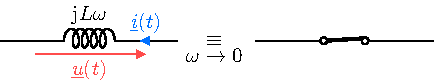
\includegraphics[width=\linewidth]{zlwa} &
    $|\ul{Z}_L| = L\w
        \underset{\w\rightarrow+\infty}{\rightarrow}+\infty$
    \smallbreak
    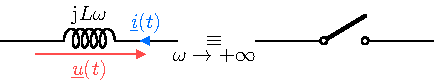
\includegraphics[width=\linewidth]{zlwi}
    \\\hline
    $|\ul{Z}_C| = 1/(C\w)
        \underset{\w\rightarrow0}{\rightarrow}+\infty$
    \smallbreak
    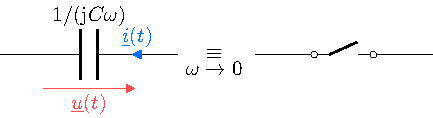
\includegraphics[width=\linewidth]{zcwa} &
    $|\ul{Z}_C| = 1/(C\w)
        \underset{\w\rightarrow+\infty}{\rightarrow}0$
    \smallbreak
    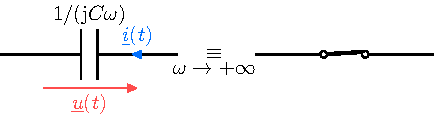
\includegraphics[width=\linewidth]{zcwi}
\end{NCprop}
En effet, l'impédance étant homogène à une résistance, on peut rendre équivalent
le fait d'avoir une impédance infinie et d'avoir une «~résistance~» infinie,
c'est-à-dire un interrupteur ouvert, qui ne laisse pas passer le courant. À
l'inverse, une résistance nulle laisse passer le courant sans résistance, comme
un fil.

\subsection{Associations d'impédances et ponts diviseurs}
Enfin, comme la relation courant-tension avec l'impédance complexe est analogue
à celle d'une résistance, on peut facilement démontrer que les associations
d'impédances suivent les associations de résistances, et qu'on peut donc
appliquer les ponts diviseurs de tension et de courant comme si on n'avait que
des résistances.

\begin{NCror}[tabularx={p{.5cm}|Y|Y}, heart]{Associations d'impédances}
    & \textbf{Schéma} & \textbf{Relations}
    \\\hline
    \rotatebox[origin=c]{90}{\textbf{En série}} &
    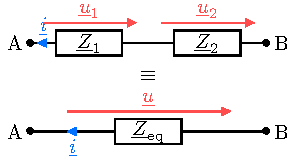
\includegraphics[width=\linewidth]{zserie} &
    \begin{bolditemize}
        \item[Impédance équivalente] :
            \[\ul{Z}_{\eq} = \ul{Z}_1 + \ul{Z}_2\]
        \item[Diviseur de tension] :
            \[\ul{u_k} = \frac{\ul{Z}_k}{\ul{Z}_{\rm branche}}\ul{u}\]
    \end{bolditemize}
    \\\hline
    \rotatebox[origin=c]{90}{\textbf{En parallèle}} &
    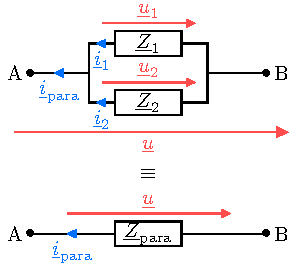
\includegraphics[width=\linewidth]{zpara} &
    \begin{bolditemize}
        \item[Dipôle équivalent] :
            \begin{gather*}
                \ul{Y}_{\eq} = \ul{Y}_1 + \ul{Y}_2\\
                \Leftrightarrow
                \frac{1}{\ul{Z}_{\eq}} = \frac{1}{\ul{Z}_1} + \frac{1}{\ul{Z}_2}\\
                \Leftrightarrow
                \ul{Z}_{\eq} = \frac{\ul{Z}_1\ul{Z}_2}{\ul{Z}_1+\ul{Z}_2}
            \end{gather*}
        \item[Diviseur de courant] :
            \begin{gather*}
                \ul{i_k} = \frac{\ul{Y}_k}{\ul{Y}_{\rm para}}\ul{i}
                \Leftrightarrow
                \ul{i_k} = \frac{\ul{Z}_{\rm para}}{\ul{Z}_k}\ul{i}\\
                \Leftrightarrow
                \ul{i_{\fbox{1}}} = \frac{\ul{Z}_{\fbox{2}}}{\ul{Z}_1 + \ul{Z}_2}\ul{i}
            \end{gather*}
    \end{bolditemize}
\end{NCror}

\subsection{Exercices bilan}
\begin{NCexem}[sidebyside, righthand ratio=.7]{Association d'impédances}
    Quelle est l'impédance de l'association suivante~?
    \begin{center}
        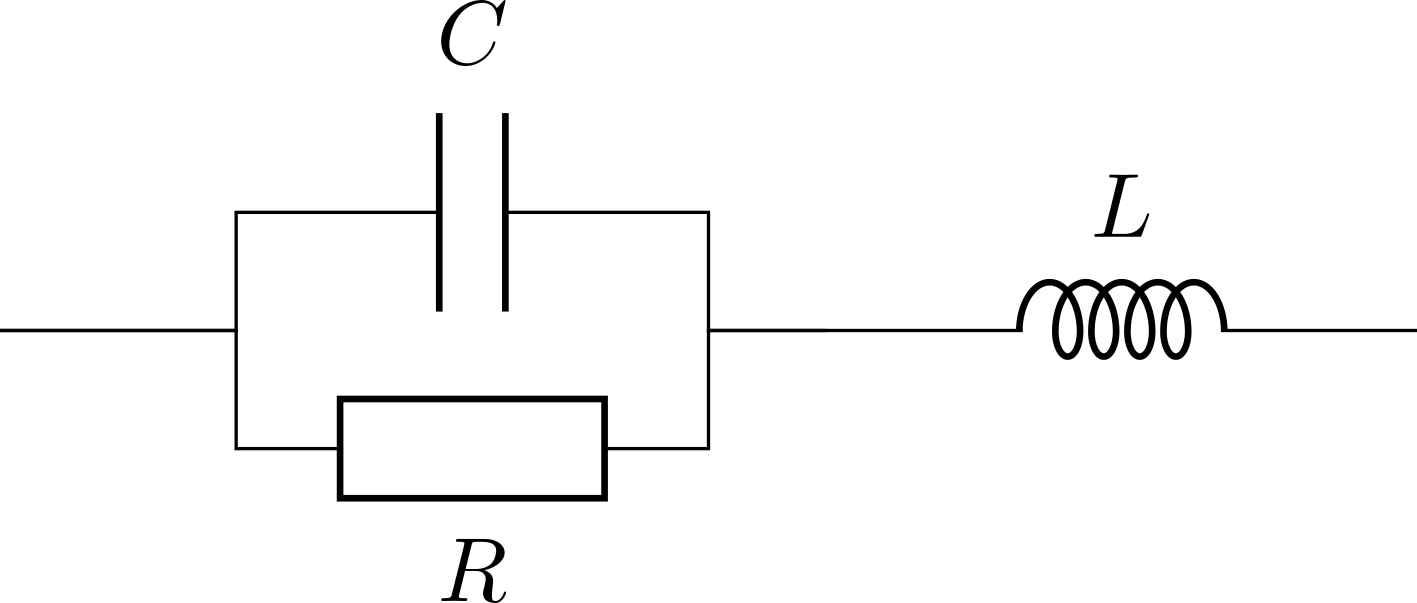
\includegraphics[width=\linewidth]{exo_zeq}
    \end{center}
    \tcblower
    L'association en parallèle donne
    $\frac{\ul{Z}_C\ul{Z}_R}{\ul{Z}_C+\ul{Z}_R}$, et on ajoute $\ul{Z}_L$ à
    celle-ci~:
    \begin{gather*}
        \ul{Z}_{\eq}
            = \frac{\dfrac{1}{\jj C\w}\times R}{\dfrac{1}{\jj C\w} + R}
                + \jj L\w
        \Leftrightarrow
        \boxed{
        \ul{Z}_{\eq} = \frac{R}{1+\jj RC\w} + \jj L\w}
    \end{gather*}
\end{NCexem}

\begin{NCexem}[valign=top]{Détermination de constantes}
    \begin{exemside}
        \vspace{-80pt}
        Soit le circuit suivant, avec une entrée sinusoïdale $e(t) = E\cos(\wt)$.
        Exprimer l'amplitude complexe $\ul{U}_C$ associée à la tension $u_C$ en fonction
        de $R$, $L$, $C$ et $\w$.
        \tcblower
        \begin{center}
            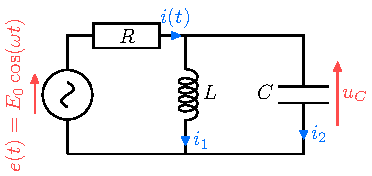
\includegraphics[width=\linewidth]{rlc_r-s-LC-parr}
        \end{center}
    \end{exemside}
    \tcblower
    S'il n'y avait pas l'inductance, on pourrait facilement utiliser un pont
    diviseur de tension pour exprimer $\ul{u}_C$ en fonction de $\ul{e}$,
    $\ul{Z}_R$ et $\ul{Z}_C$. Pour se ramener à la situation du pont diviseur de
    tension, on détermine donc une première impédance équivalente issue de
    l'association en parallèle de $L$ et $C$, après les avoir converties en
    complexes~:
    \begin{center}
        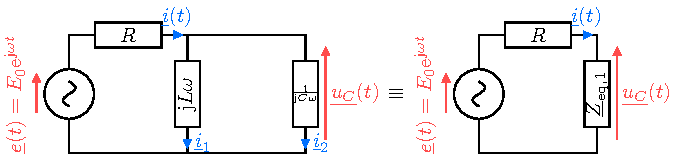
\includegraphics[width=\linewidth]{rlc_r-s-LC-parr_cplx}
    \end{center}
    On peut déterminer $\ul{Z}_{\eq, 1}$ avec les admittances $\ul{Y}_L = 1/\jj
    L \w$ et $\ul{Y}_C = \jj C\w$, et utiliser le pont diviseur de tension
    directement avec l'amplitude complexe~: $\ul{U}_C =
    \frac{\ul{Z}_{\eq,1}}{\ul{Z}_{\eq,1}+\ul{Z}_R}E_0$. Ainsi,
    \begin{gather*}
        \ul{U}_C = \frac{\dfrac{1}{
            \color{orange}\cancel{\dfrac{1}{\jj L\w} + \jj C\w}}}
            {\dfrac{1}{\textcolor{orange}{\cancel{\dfrac{1}{\jj L\w} + \jj C\w}}}
            + R\color{orange}(…)}E_0
            \times \textcolor{orange}{
                \frac{\jj C\w + \dfrac{1}{\jj L\w}}{\jj C\w + \dfrac{1}{\jj L\w}}}
        \Leftrightarrow
        \ul{U}_C = \frac{1}{1 + \jj RC\w + \dfrac{R}{\jj L\w}}E_0\\
        \Leftrightarrow
        \boxed{
            \ul{U}_C = \frac{E_0}{1 + \jj \left( RC\w - \dfrac{R}{L\w} \right)}
        }
    \end{gather*}
    où on a simplifié la fraction en multipliant par le terme orange d'abord,
    puis en utilisant que $1/\jj = -\jj$.
\end{NCexem}

\subsection{Résumé}

\begin{rror}{Résumé méthode}
    Un système soumis à une excitation sinusoïdale du type $e(t) = E_O\cos(\wt)$ se
    comporte de la manière suivante~:
    \begin{itemize}
        \item Après un court régime transitoire (solution homogène), les signaux de
            sortie seront eux aussi sinusoïdaux et \textbf{à la même pulsation}, de
            la forme $x(t) = X\cos(\wt+\f_X)$~: le RSF correspond à l'étude de ces
            fonctions (solutions particulières) dont l'amplitude $X$ et la phase
            $\f_X$ sont définies \textbf{par le système} (et non pas des conditions
            initiales).
        \item Pour trouver ces valeurs, on définit~:
            \begin{itemize}
                \item \leftcenters{l'entrée complexe~:}{$\ul{e}(t) =
                    E\exr^{\jj\wt}$}
                \item les signaux de sortie complexes~: $\ul{x}(t) =
                    X\exr^{\jj(\wt+\f_X)}$~;
                \item les amplitudes complexes $\ul{X} = X\exr^{\jj\f_X}$,
                    telles que $\ul{x}(t) = \ul{X}\exr^{\jj\wt}$~;
                \item On retrouve les grandeurs réelles en en prenant le module et
                    la phase~:
                    \[ \boxed{X = \left| \ul{X} \right|}
                        \qet
                        \boxed{\f_X = \arg(\ul{X})}
                    \]
            \end{itemize}
    \end{itemize}
\end{rror}

\section{Mesure de déphasages}
\subsection{Définition}
\begin{NCdefi}[width=\linewidth]{Définition~: déphasage}
    Pour deux signaux sinusoïdaux $s_1(t) = S_1\cos(\w_1t+\f_1)$ et $s_2(t) =
    S_2\cos(\w_2t+\f_2)$, on définit le \textbf{déphasage} entre $s_2$ et $s_1$
    comme étant la \textbf{différence de leurs phases instantanées}~:
    \[\D\f_{2/1} = (\w_1t + \f_2) - (\w_2t+\f_1)\]
    Pour de signaux \textit{de même fréquence}, le déphasage est simplement la
    \textbf{différence des phases à l'origine des temps}~:
    \[\boxed{\D\f_{2/1} = \f_2 - \f_1}\]
\end{NCdefi}
\begin{rrapp}{\includehand{-90}{0.8cm}}
    Étant donné que les sorties en RSF ont la même pulsation que l'entrée, on ne
    s'intéressera qu'à des signaux de même pulsation/fréquence.
\end{rrapp}

\vspace{-20pt}
\subsection{Valeurs particulières}
\subsubsection{Signaux en phase}
\vspace{-20pt}
\begin{minipage}{0.70\linewidth}
    \begin{rdefi}{\small Définition}
        Deux signaux sont en phase si leur déphasage est nul (modulo $2\pi$)~:
        \[\boxed{\D\f \equiv 0\quad[2\pi]}\]
        Les signaux passent par leurs valeurs maximales et minimales aux mêmes
        instants, et s'annulent simultanément.
    \end{rdefi}
\end{minipage}
\hfill
\begin{minipage}{0.30\linewidth}
    \begin{center}
        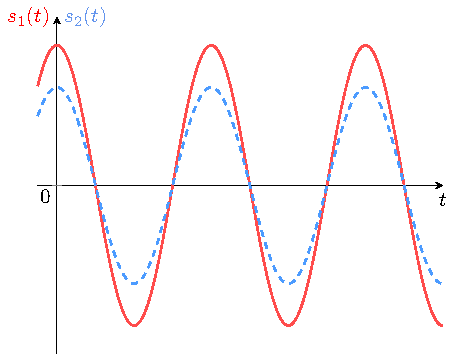
\includegraphics[width=\linewidth]{dfeq0.pdf}
    \end{center}
\end{minipage}

\vspace{-20pt}
\subsubsection{Signaux en quadrature de phase}

\begin{minipage}{0.70\linewidth}
    \begin{rdefi}{\small Définition}
        Deux signaux sont en quadrature phase si leur déphasage est de
        $\pm\pi/2$ (modulo $2\pi$)~:
        \[\boxed{\D\f \equiv \pm\frac{\pi}{2} \quad[2\pi]}\]
        Quand un signal s'annule, l'autre est à son maximum où à son minimum~:
        c'est la relation entre un cosinus et un sinus.
    \end{rdefi}
\end{minipage}
\hfill
\begin{minipage}{0.30\linewidth}
    \begin{center}
        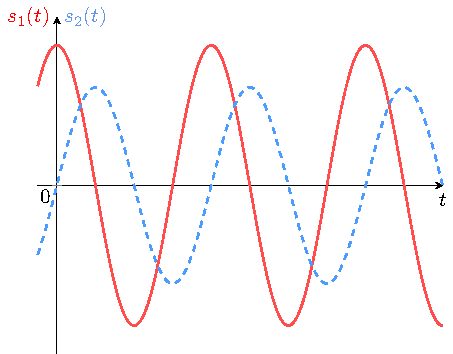
\includegraphics[width=\linewidth]{dfeqpi2.pdf}
    \end{center}
\end{minipage}

\newpage
\subsubsection{Signaux en opposition de phase}

\begin{minipage}{0.70\linewidth}
    \begin{rdefi}{\small Définition}
        Deux signaux sont en phase si leur déphasage est de $\pm\pi$ (modulo $2\pi$)~:
        \[\boxed{\D\f \equiv \pm\pi \quad[2\pi]}\]
        Lorsqu'un signal passe par sa valeur maximale, l'autre est à la valeur
        minimale, mais ils s'annulent simultanément.
    \end{rdefi}
\end{minipage}
\hfill
\begin{minipage}{0.30\linewidth}
    \begin{center}
        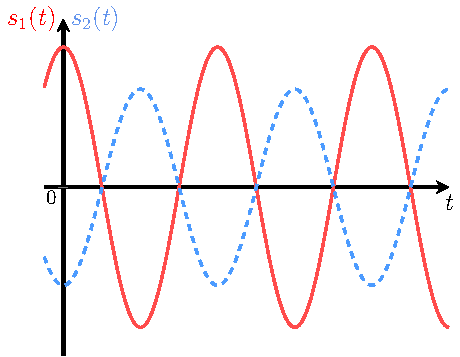
\includegraphics[width=\linewidth]{dfeqpi.pdf}
    \end{center}
\end{minipage}

\subsection{Lecture d'un déphasage}
Le déphasage $\D\f_{2/1} = \f_2 - \f_1$ est lié au \textbf{retard temporel}
$\tau_{1/2}$ du signal $s_1$ par rapport au signal $s_2$~: on a
\[\boxed{\D\f_{2/1} = \w\tau_{1/2}}\]

\begin{minipage}{0.70\linewidth}
    Dans ce cas, le déphasage obtenu est entre $-\pi$ et $+\pi$. On définit alors~:
    \begin{itemize}
        \item $\D\f_{2/1} > 0 \Rightarrow s_2$ est en avance sur $s_1$~;
        \item $\D\f_{2/1} < 0 \Rightarrow s_2$ est en retard sur $s_1$.
    \end{itemize}
\end{minipage}
\begin{minipage}{0.30\linewidth}
    \begin{center}
        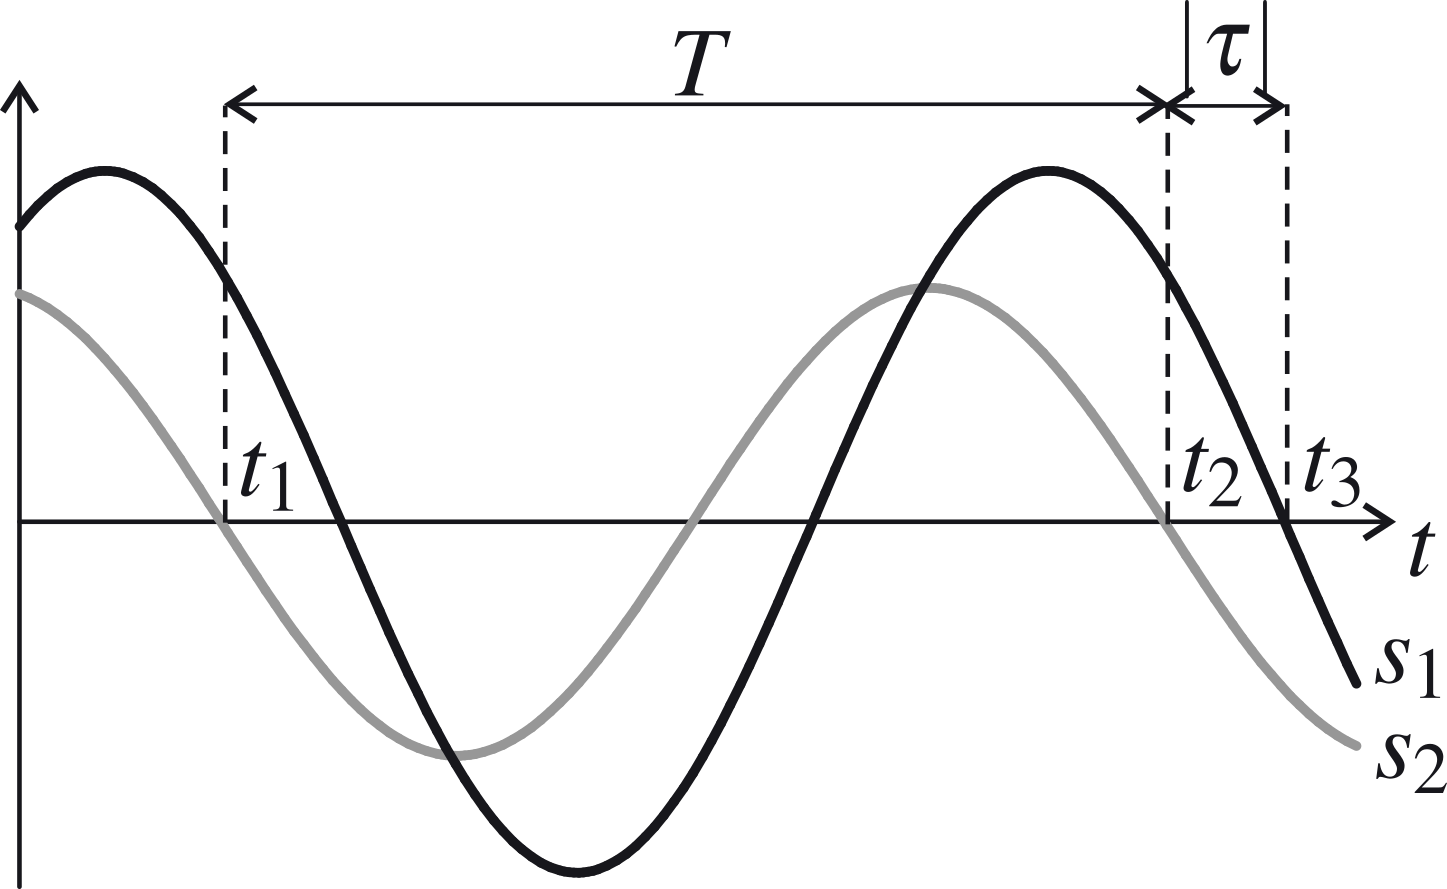
\includegraphics[width=\linewidth]{dfretard}
    \end{center}
\end{minipage}

Le principe est de mesurer la différence de temps entre les deux moments les
plus proches tels que les deux signaux s'annulent \textbf{avec la même pente}.
Par construction, la pulsation représente une vitesse angulaire, c'est pourquoi
on a $\w = 2\pi/T$ comme $v = d/t$ en mécanique. On trouve donc naturellement la
relation entre $\D\f_{2/1}$ et $\tau_{2/1}$.

\subsection{Déphasage des impédances}
Pour un dipôle de tension $\ul{U}$ traversé par une intensité $\ul{I}$, on
définit $\ul{Z} = \frac{\ul{U}}{\ul{I}}$, et on a donc $\arg(\ul{Z}) =
\arg(\ul{U}) - \arg(\ul{I})$. Ainsi, la phase d'une impédance représente le
déphasage entre la tension et le courant. Pour les différents dipôles
classiques, on trouve~:
\begin{itemize}
    \item $\arg(\ul{Z}_R) = 0 \Rightarrow$ signaux en phase~;
    \item $\arg(\ul{Z}_L) = \arg(\jj L\w) = \pi/2 \Rightarrow$ signaux en
        quadrature de phase, avec $\ul{u}$ en avance sur $\ul{i}$~;
    \item $\arg(\ul{Z}_C) = \arg(1/\jj C\w) = -\pi/2 \Rightarrow$ signaux en
        quadrature de phase, avec $\ul{u}$ en retard sur $\ul{i}$~;
\end{itemize}

\end{document}
